\chapter{Introduction}
\label{ch:introduction}

This is a very short guide to an unofficial thesis/dissertation template for the
Department of Statistics \& Data Science at Carnegie Mellon University. This
template was created by Alex Reinhart, drawing upon an earlier template adapted
by Heidi Sestrich from a template used by the University of Tennessee,
Knoxville. That template was modified with the kind permission of its author, T.
Saad.

This template requires a basic knowledge of \LaTeX\ and should cover the basic
requirements in terms of required packages and functionality. There are a few
useful resources if you need \LaTeX\ help:
\begin{itemize}
\item The \href{https://en.wikibooks.org/wiki/LaTeX}{LaTeX Wikibook}, a full
  guide to \LaTeX
\item The
  \href{http://mirrors.ctan.org/macros/latex/required/amsmath/amsldoc.pdf}{amsmath
    manual} describes the mathematical features provided by the amsmath package:
  aligned equations, multiline equations, matrices, arrows, special symbols and
  characters, and so on.
\item The
  \href{http://mirrors.ctan.org/macros/latex/contrib/memoir/memman.pdf}{memoir
    class manual}. This template is based on the memoir class, and memoir has
  options for styling, sizing, layout, and so on, and a very thorough manual.
\end{itemize}

\section{Disclaimer}

This template is distributed with ABSOLUTELY NO WARRANTY. It serves as a
guideline and constitutes a basic structure for a thesis/dissertation. The user
assumes full responsibility for formatting and typesetting their document and
for verifying that all the thesis requirements set by the Department of
Statistics \& Data Science are met. Please refer to the most recent CMU
Statistics PhD handbook.

\section{Getting started}

This template uses several folders:
\begin{description}
\item[front-matter] The signature page, abstract, and similar material
\item[chapters] The main text of your thesis, with one \LaTeX\ file per chapter
\item[back-matter] Appendices, such as the Data and Code Availability appendix
\item[figures] Any figures you include, in PDF, PNG, JPEG, or similar format.
  (PDF is recommended for plots and line art.)
\end{description}

Note that this is only a suggested model that could be modified to fit your own
organizational structure.

The \texttt{thesis.tex} file is the main file for your thesis/dissertation. This
is where you should start editing and planning for your thesis/dissertation. You
may want to change the name of the file to something like
\texttt{my-name-thesis.tex}. Next, fill in the information at the top of the
file, including your thesis title, date, advisor, committee members, and so on;
comments in the file explain how to do it. This is the file you will compile to
produce your PDF.

The class file \texttt{cmustatthesis.cls} contains the settings, definitions,
packages, and macros for this template to work properly and is located in the
root directory. This file constitutes the document class for the template. It is
based on the memoir class and provides some customized functionality. For
example, it can automatically generate the signature page and title page for
you, based on the CMU requirements. You should not need to modify the class
file.

\textbf{Important note:} If you decide to change anything about this template,
such as adjusting margins, headers, chapter and section title styling, or any
other such details, \textbf{check the
  \href{http://mirrors.ctan.org/macros/latex/contrib/memoir/memman.pdf}{memoir
    manual} first.} The memoir document class is comprehensive and has options
for \emph{everything}. If you instead Google how to do something, and use the
first code you find on the \TeX\ Stack Exchange, you may end up using packages
that conflict with memoir and cause unexpected problems. The memoir manual is
\emph{extremely} thorough, so you should use it as your first reference.

In certain cases, one of the packages included in this template may conflict
with a package that you are adding. You will have to resolve this conflict by
either removing the package that is not being used or by modifying some settings
with either packages. The packages that are preloaded in this class file are:
amsmath, amsthm, amssymb, setspace, geometry, hyperref, and color.

\section{References}

We recommend using BibTeX for your references. This template is set up to use
\href{http://mirrors.ctan.org/macros/latex/contrib/natbib/natbib.pdf}{the natbib
  package} for bibliography management, using the ``apalike'' reference style.

The \texttt{thesis-references.bib} file contains some example BibTeX entries. To
cite, use the \verb|\citet| command to use a reference in a sentence, and use
\verb|\citep| for a parenthetical citation. For example, \citet{Wasserman:2004}
is a common statistics reference, and I've cited it here with \verb|\citet|.
Alternately, we often put references in parentheses using \verb|\citep|
\citep{Underhill:1999}.

\section{Cross-referencing}

\LaTeX\ can automatically insert cross-reference link to figures, tables,
sections, equations, theorems, and so on. Use \verb|\label| to give something a
name (such as a figure or section), and then use \verb|\ref| to refer to it. For
instance, this chapter begins with
\begin{verbatim}
\chapter{Introduction}
\label{ch:introduction}
\end{verbatim}
We can hence refer to it with \verb|Chapter \ref{ch:introduction}|, producing
Chapter \ref{ch:introduction}.

When using the \verb|equation| environment or similar environments, \LaTeX\ will
automatically number equations. (Use starred versions, like \verb|equation*|, to
have it not insert numbers.) You can cross-reference these too, again using
\verb|\label|. But instead of \verb|\ref|, use \verb|\eqref|, which typesets the
number in parentheses to match how it is displayed next to the equation. For
example, in the next section you can find equation \eqref{eq:risk}.

\section{Basic mathematics}

Try to use built-in \LaTeX\ features for math, rather than doing things
yourself. For instance, compare the two equations below:
\begin{align*}
  sin^2 \theta + cos^2 \theta &= 1\\
  \sin^2 \theta + \cos^2 \theta &= 1.
\end{align*}
Using \verb|\sin| instead of \verb|sin| ensures it is typeset as an operator,
not as the variables $s$, $i$, and $n$ multiplied together. This also ensures
correct spacing.

The
\href{http://mirrors.ctan.org/macros/latex/required/amsmath/amsldoc.pdf}{amsmath
  package} provides many useful mathematical features, and you should consider
reviewing its manual. For example, you can declare new mathematical operators by
using \verb|\DeclareMathOperator| in your preamble:\verbfootnote{Preamble means
  ``before \verb|\begin{document}| in \texttt{thesis.tex}.''}
\begin{verbatim}
\DeclareMathOperator{\E}{\mathbb{E}}
\DeclareMathOperator{\logit}{logit}
\end{verbatim}
Now we can write \verb|\E| and \verb|\logit| to get these typeset as operators,
instead of having to write out \verb|\mathbb{E}| or \verb|\text{logit}| every
time we use them. For one-off operators, you can use \verb|\operatorname|:
\begin{equation}\label{eq:risk}
  R = \operatorname{risk}(\hat f).
\end{equation}
Unlike \verb|\def| or \verb|\newcommand|,
\verb|\DeclareMathOperator| is specialized for mathematical operators and sets
up spacing, font, and positioning of superscripts and subscripts.

amsmath also makes formula typesetting easy. For instance, the \texttt{align}
environment for aligning equations:
\begin{align*}
  \lambda(t \mid \mathcal{H}_t) &= \nu + \int_0^t g(t - u) \, d N(u)\\
                             &= \nu + \sum_{i: t_i < t} g(t - t_i).
\end{align*}
We recommend using \texttt{align} rather than the old \texttt{eqnarray}, which
has poor spacing. (Here we've used \texttt{align*}, which does not number each
equation.)

amsmath also provides features for splitting long equations across multiple
lines, and for typesetting matrices, piecewise function definitions, and so on.
Check
\href{http://mirrors.ctan.org/macros/latex/required/amsmath/amsldoc.pdf}{its
  manual} for more details.


\section{Theorem and definition environments}

This template contains predefined theorem, lemma, corollary, and definition
environments. These are numbered and can optionally have names. For example:
\begin{theorem}[Doe's Law]\label{thm:theorem-a}
  This is an example theorem.
\end{theorem}
\begin{proof}[Proof for theorem \ref{thm:theorem-a}]
  This is the proof for this theorem.
\end{proof}

\begin{lemma}[First lemma]
  This is the first lemma.
\end{lemma}
\begin{corollary}
  This is the first corollary.
\end{corollary}

\begin{definition}[Schervish def.\ 2.39]
  A statistic \(U\) is called \emph{ancillary} if the conditional distribution
  of \(U\) given \(\Theta = \theta\) is the same for all \(\theta\).
\end{definition}
We can easily cross-reference numbered theorems and definitions, such as
Theorem~\ref{thm:theorem-a}.

\section{Figures}

For more information, check
\href{https://en.wikibooks.org/wiki/LaTeX/Floats,_Figures_and_Captions}{the
  LaTeX Wikibook}. The basic way to include a figure is like this:

\begin{verbatim}
\begin{figure}
    \centering % center the figure
    \includegraphics[width=\textwidth]{figure-name}
    \caption[optional short caption for List of Figures]{
      Full figure caption with explanation, printed under
      the figure on the page
    }
    \label{figure-label}
\end{figure}
\end{verbatim}

Notice the use of \verb|\textwidth| to set the width of the figure. This makes
the figure as wide as the text block. You can also use a multiple of
\verb|\textwidth|, such as \verb|0.5\textwidth|, or an absolute size like
\texttt{3in} or \texttt{10cm}.

\begin{figure}
  \centering
  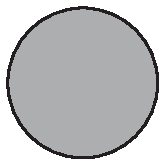
\includegraphics[width=0.5\textwidth]{fig02a-circle}
  \caption[Short caption for LoF]{Sample caption.}
  \label{label}
\end{figure}

Do \textbf{not} try to get into a fight with \LaTeX\ over where it places
figures. You will lose, and gain a lot of frustration in the process. \LaTeX\
will place figures automatically, typically at the top or bottom of pages. It is
standard style in academic writing to let the figures float to the top of pages,
rather than embedding them in your text, and then to refer to them by number.
For instance, as you can see in Figure~\ref{label}, circles are round.

\section{Tables}

There are a few useful stylistic rules to remember for tables:
\begin{itemize}
\item There is no point to having vertical lines between every column or
  horizontal lines between every row.
\item Text should be left-aligned, since we are used to reading left-aligned
  text.
\item Numbers should be \textbf{right}-aligned and presented with the same
  number of decimal places when possible. This makes it easy to compare the size
  of different numbers.
\end{itemize}

The booktabs package provides some nice formatting features for tables, and is
automatically loaded in this thesis template. Table~\ref{sample-table} is a
sample of a table formatted this way. Check Chapter 11 of the
\href{http://mirrors.ctan.org/macros/latex/contrib/memoir/memman.pdf}{memoir
    manual} for additional table formatting information.

\begin{table}
  \centering
  \begin{tabular}{l r r}\toprule
    Text column & Number 1 & Number Dos \\\midrule
    Foo & 10.0 & 0.1 \\
    Bar & 1.2 & 27.4 \\
    Baz & 0.8 & 1341.0 \\\bottomrule
  \end{tabular}
  \caption[Demonstration booktabs table]{A sample table. Notice how the
    right-aligned numbers are easy to compare, since the decimal points line
    up.}
  \label{sample-table}
\end{table}

If you are using R to generate tables, there are two good options. The
\href{https://gt.rstudio.com/}{gt} package supports very fancy tables; knitr's
\texttt{kable()} function can also output \LaTeX\ tables from data frames, and
the \texttt{booktabs = TRUE} option will make it use booktabs.

\section{Special characters}

Versions of \LaTeX\ installed since 2019 automatically support UTF-8 characters
in input files, meaning you can directly insert accented characters into the
file. För ïńštånçe, like this.

However, particular fonts may not support particular characters. Two of the
characters in the previous paragraph do not appear when this document is typeset
using the Latin Modern (default) font, for example, and the log file has
messages saying
\begin{verbatim}
Missing character: There is no ń ("144) in font ec-lmr10!
Missing character: There is no š ("161) in font ec-lmr10!
\end{verbatim}
(The characters may not show up here either.) If you need characters not
provided in the font you are using, you may need to try switching to a different
font.
